\section*{Plan de Trabajo}

\subsection*{Descripción general del trabajo}

El presente Trabajo de Fin de Grado, tiene como objetivo el diseño e implementación de un sistema informático para el análisis y la predicción temporal del rendimiento de fondos de inversión, empleando técnicas de análisis de datos y Machine Learning. 

El proyecto abordará el ciclo completo de un sistema de datos, desde la adquisición y el almacenamiento estructurado de información histórica de fondos, variables financieras y macroeconómicas, hasta su posterior procesamiento. Sobre estos datos se aplicarán técnicas de análisis estadístico y aprendizaje automático, trabajando con series temporales multivariantes para estudiar tendencias, patrones y relaciones entre variables, lo que permitirá generar predicciones periódicas del comportamiento de los fondos a distintos horizontes temporales (1, 3, 6 meses …). 

El sistema desarrollado posibilitará la comparación de distintos modelos predictivos, evaluando su rendimiento mediante métricas cuantitativas y visualizando los resultados para garantizar la reproducibilidad y trazabilidad del proceso. Adicionalmente, se incorporará un módulo de simulación de escenarios hipotéticos para analizar el comportamiento del mercado ante distintos contextos macroeconómicos (como crisis o cambios en tipos de interés). 

Para reforzar la validez del análisis, se emplearán técnicas de interpretabilidad de modelos (SHAP y LIME) que permitan analizar la influencia de las variables utilizadas y justificar las predicciones obtenidas.

\subsection*{Lista de objetivos}

\begin{itemize}
    \item Obtención y gestión de datos: recopilación de históricos financieros y macroeconómicos, y diseño de BD.
    \item Procesamiento: adquisición, limpieza, transformación e integración de datos para estudiar tendencias y relaciones.
    \item Generación de nuevas variables y preparación de dataset multivariante.
    \item Desarrollo de modelos predictivos: Machine Learning (explicabilidad) y Deep Learning (precisión).
    \item Predicciones a 1, 3 y 6 meses con evaluación de precisión.
    \item Backtesting y comparación de modelos (con/sin variables macroeconómicas).
    \item Técnicas de interpretabilidad (SHAP, LIME) para explicar predicciones.
    \item Documentación y visualización de resultados.
\end{itemize}

\subsection*{Lista de actividades}

\begin{itemize}
    \item \textbf{Tarea 1 - Planificación del proyecto}: plan de trabajo, alcance, horas.
    \item \textbf{Tarea 2 — Estudio teórico}: análisis financiero, series temporales, ML/DL, modelos predictivos.
    \item \textbf{Tarea 3 — Estudio del dominio}: mercados, fondos de inversión, variables macro, fuentes de datos, herramientas (Python, R, SHAP, LIME...).
    \item \textbf{Tarea 4 — Diseño del sistema}: datastream, pipeline, BD, diccionario de datos.
    \item \textbf{Tarea 5 — Recolección y preparación}: obtención de datos, limpieza, transformación, dataset final.
    \item \textbf{Tarea 6 — Análisis de datos}: tendencias, volatilidad, correlaciones, variables derivadas.
    \item \textbf{Tarea 7 — Desarrollo de modelos}: entrenamiento/validación, modelos base, ML (Random Forest, Gradient Boosting), DL (LSTM multivariante-multistep), backtesting.
    \item \textbf{Tarea 8 — Evaluación y simulación}: comparación de modelos, experimentos con/sin macro, escenarios what-if.
    \item \textbf{Tarea 9 — Interpretabilidad y visualización}: SHAP, LIME, importancia de variables, gráficos y dashboards.
    \item \textbf{Tarea 10 — Documentación y defensa}: memorias de seguimiento y final, presentación y guión.
\end{itemize}

\subsection*{Diagrama de Gantt}

\begin{figure}[htbp]
    \centering
    \includegraphics[width=1\textwidth]{imagenes/diagramaGantt.png}
    \caption{Diagrama de Gantt con la planificación temporal del proyecto}
    \label{fig:diagramaGantt}
\end{figure}

\newpage

\subsection*{Propuesta del tutor}
\begin{figure}[htbp]
    \centering
    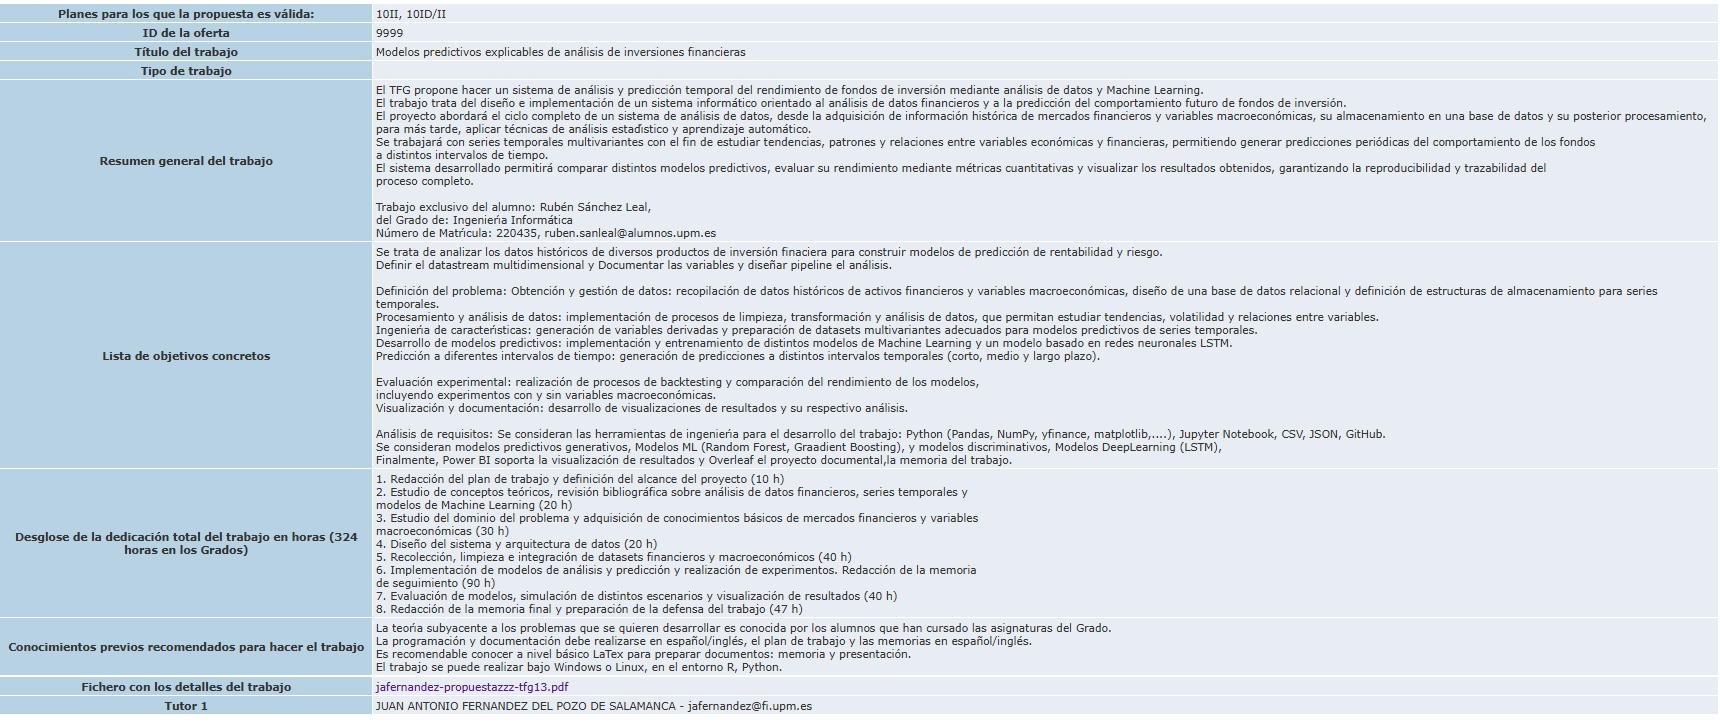
\includegraphics[width=1\textwidth]{imagenes/propuestaTutor.png}
    \caption{Propuesta del tutor Rubén Sánchez Leal}
    \label{fig:propuestaTutor}
\end{figure}